\documentclass[
11pt, % The default document font size, options: 10pt, 11pt, 12pt
%codirector, % Uncomment to add a codirector to the title page
]{charter} 
\usepackage{slashbox}

% El títulos de la memoria, se usa en la carátula y se puede usar el cualquier lugar del documento con el comando \ttitle
\titulo{Identificación de documentos con reconocimiento de caracteres} 

% Nombre del posgrado, se usa en la carátula y se puede usar el cualquier lugar del documento con el comando \degreename
%\posgrado{Carrera de Especialización en Sistemas Embebidos} 
%\posgrado{Carrera de Especialización en Internet de las Cosas} 
\posgrado{Carrera de Especialización en Inteligencia Artificial}
%\posgrado{Maestría en Sistemas Embebidos} 
%\posgrado{Maestría en Internet de las cosas}

% Tu nombre, se puede usar el cualquier lugar del documento con el comando \authorname
% IMPORTANTE: no omitir titulaciones ni tildación en los nombres, también se recomienda escribir los nombres completos (tal cual los tienen en su documento)
\autor{Ing. Viñas, Gustavo José Miguel}

% El nombre del director y co-director, se puede usar el cualquier lugar del documento con el comando \supname y \cosupname y \pertesupname y \pertecosupname
\director{Título y Nombre del director}
\pertenenciaDirector{pertenencia} 
\codirector{} % para que aparezca en la portada se debe descomentar la opción codirector en los parámetros de documentclass
\pertenenciaCoDirector{FIUBA}

% Nombre del cliente, quien va a aprobar los resultados del proyecto, se puede usar con el comando \clientename y \empclientename
\cliente{Landeira Daniel}
\empresaCliente{Asyst S.A.}
 
\fechaINICIO{29 de abril de 2025}		%Fecha de inicio de la cursada de GdP \fechaInicioName
\fechaFINALPlan{17 de junio de 2025} 	%Fecha de final de cursada de GdP
\fechaFINALTrabajo{mes de abril de 2026}	%Fecha de defensa pública del trabajo final


\begin{document}

\maketitle
\thispagestyle{empty}
\pagebreak


\thispagestyle{empty}
{\setlength{\parskip}{0pt}
\tableofcontents{}
}
\pagebreak


\section*{Registros de cambios}
\label{sec:registro}


\begin{table}[ht]
\label{tab:registro}
\centering
\begin{tabularx}{\linewidth}{@{}|c|X|c|@{}}
\hline
\rowcolor[HTML]{C0C0C0} 
Revisión & \multicolumn{1}{c|}{\cellcolor[HTML]{C0C0C0}Detalles de los cambios realizados} & Fecha      \\ \hline
0      & Creación del documento                                 &\fechaInicioName \\ \hline
1      & Se completa hasta el punto 5 inclusive                & {13} de {mayo} de 2025 \\ \hline
1.1      & Correcciones versión 1                & {17} de {mayo} de 2025 \\ \hline
2      & Se completa hasta el punto 9 inclusive                  & {20} de {mayo} de 2025 \\ \hline
%3      & Se completa hasta el punto 12 inclusive                & {27} de {mayo} de 2025 \\ \hline
%4      & Se completa el plan	                                 & {03} de {junio} de 2025 \\ \hline

% Si hay más correcciones pasada la versión 4 también se deben especificar acá

\end{tabularx}
\end{table}

\pagebreak



\section*{Acta de constitución del proyecto}
\label{sec:acta}

\begin{flushright}
Buenos Aires, \fechaInicioName
\end{flushright}

\vspace{2cm}

Por medio de la presente se acuerda con el \authorname\hspace{1px} que su Trabajo Final de la \degreename\hspace{1px} se titulará ``\ttitle'' y consistirá en ubicar el área de datos de interés en documentos que poseen un formato específico, para reconocer y validar tres líneas de caracteres que lo identifican de forma unívoca. El trabajo tendrá un presupuesto preliminar estimado de 600 horas y un costo estimado de U\$S 15.000, con fecha de inicio el \fechaInicioName\hspace{1px} y fecha de presentación pública en el \fechaFinalName.

Se adjunta a esta acta la planificación inicial.

\vfill

% Esta parte se construye sola con la información que hayan cargado en el preámbulo del documento y no debe modificarla
\begin{table}[ht]
\centering
\begin{tabular}{ccc}
\begin{tabular}[c]{@{}c@{}}Dr. Ing. Ariel Lutenberg \\ Director posgrado FIUBA\end{tabular} & \hspace{2cm} & \begin{tabular}[c]{@{}c@{}}\clientename \\ \empclientename \end{tabular} \vspace{2.5cm} \\ 
\multicolumn{3}{c}{\begin{tabular}[c]{@{}c@{}} \supname \\ Director del Trabajo Final\end{tabular}} \vspace{2.5cm} \\
\end{tabular}
\end{table}




\section{1. Descripción técnica-conceptual del proyecto a realizar}
\label{sec:descripcion}

Asyst S.A., una empresa con 35 años de experiencia en la captura y procesamiento de documentos en el ámbito bancario, tiene clientes a los que les ha desarrollado sistemas de carga de datos manual a partir de imágenes. Años atrás, la empresa ensayó soluciones de reconocimiento de caracteres para estos sistemas (sin utilizar inteligencia artificial) con resultados por debajo de la expectativa esperada. En la actualidad, busca expandir sus horizontes e incluir herramientas de inteligencia artificial que mejoren los resultados y faciliten la tarea a los clientes.


Si bien existen soluciones genéricas para el reconocimiento de documentos y caracteres, aplicarlos sobre todo el documento no resulta conveniente, debido a la cantidad de información extraída, el posprocesamiento que esto implica, y la baja tasa de reconocimiento del área de interés.

El proyecto consiste en el procesamiento de documentos mediante imágenes, con el objetivo de obtener los datos que lo identifican, ubicados en un área determinada. 

A partir de las imágenes capturadas, las que podrán ser a color o blanco y negro, se buscará identificar el rectángulo que contiene información relevante. Dentro de este rectángulo se encuentran 3 líneas (de números, espacios y guiones), con dos tipografías predominantes, aunque no exclusivas, a las que se les aplicará reconocimiento de caracteres.\\
Cada una de ellas cuenta con un dígito verificador, que se validará y definirá si los datos identificados son correctos.

La información relevante también se encuentra en una línea inferior del documento, con una tipografía específica (distinta a las anteriores), con un dígito especial de inicio y otro de fin, sin dígitos verificadores.
Será parte de este proyecto, analizar y utilizar esta información, si fuera útil para mejorar el resultado.

En la figura \ref{fig:diagBloques} se puede observar el diagrama en bloques.

El proyecto tendrá en cuenta que el rectángulo o área de interés puede verse afectado por trazos que invadan la zona, o por fondos que pueden perjudicar el reconocimiento. Por ese motivo, la solución contemplará el preprocesamiento de la imagen para eliminar o minimizar dicho ruido.

El conjunto de datos contiene información privada que no podrá ser publicada sin antes anonimizar o difuminar.

\begin{figure}[htpb]
\centering 
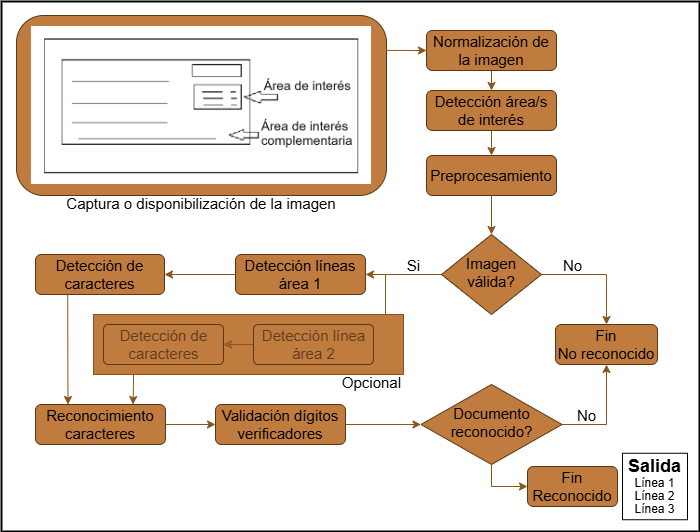
\includegraphics[width=.94\textwidth]{./Figuras/diagBloques.png}
\caption{Diagrama en bloques del sistema.}
\label{fig:diagBloques}
\end{figure}

\vspace{25px}

\section{2. Identificación y análisis de los interesados}
\label{sec:interesados}

\begin{table}[ht]
%\caption{Identificación de los interesados}
%\label{tab:interesados}
\begin{tabularx}{\linewidth}{@{}|l|X|X|l|@{}}
\hline
\rowcolor[HTML]{C0C0C0} 
Rol           & Nombre y Apellido & Organización 	& Puesto 	\\ \hline
Cliente       & \clientename      &\empclientename	& Presidente \\ \hline
Responsable   & \authorname       & FIUBA        	& Alumno 	\\ \hline
Orientador    & \supname	      & \pertesupname 	& Director del Trabajo Final \\ \hline
\end{tabularx}
\end{table}

\begin{itemize}
	\item Cliente: el señor Landeira es exigente con la calidad de los desarrollos. Una de sus prioridades es que los productos, al llegar al usuario final, no tengan defectos. Se preocupa por mantener una imagen positiva de la empresa.
	\item Orientador: a definir.
\end{itemize}

\newpage
\section{3. Propósito del proyecto}
\label{sec:proposito}

Automatizar el ingreso de datos que identifican el documento, reduciendo la carga manual, el tiempo y los costos operativos asociados.


\section{4. Alcance del proyecto}
\label{sec:alcance}

El presente proyecto comprende:
\begin{itemize}
	\item Preprocesamiento de la imagen.
	\item Identificación del área de interés.
	\item Normalización de la imagen.
	\item Reconocimiento de caracteres.
	\item Validación del resultado obtenido.
	\item Análisis de performance de la solución.
	\item Análisis y selección del conjunto de datos.
\end{itemize}

El presente proyecto no incluye:
\begin{itemize}
	\item Captura de imágenes.
	\item Incorporación a soluciones existentes.
	\item La extensión de reconocimiento sobre otras áreas de interés presentes en el documento.
\end{itemize}

\section{5. Supuestos del proyecto}
\label{sec:supuestos}

Para el desarrollo del presente proyecto se establece que:
\begin{itemize}
	\item El conjunto de datos aportado por el cliente será suficiente para realizar el entrenamiento.
	\item El cliente pondrá a disposición la información requerida en tiempo y forma.
	\item Los recursos de hardware y software requeridos para llevar a cabo este proyecto serán proporcionados por el cliente. El responsable del proyecto podrá aportar los recursos que tuviese disponibles, siempre que exista acuerdo con el cliente.
	\item La solución obtenida debe ser eficiente en el tiempo de reconocimiento.
	\item La solución obtenida debe ser mejor que aplicar al documento un transformer multimodal como chatGPT, u otros modelos similares.
\end{itemize}


\section{6. Product Backlog}
\label{sec:backlog}

\textbf{Criterio para la estimación de Story Points:} cada historia de usuario se evalúa en tres dimensiones fundamentales (dificultad, complejidad e incertidumbre) con puntuaciones según se muestra en el cuadro \ref{tab:storypoints}. Estos valores son sumados y redondeados al número más cercano (igual o superior) de la secuencia de Fibonacci (0, 1, 2, 3, 5, 8, 13, 21, 34).

\begin{table}[ht]
\caption{Evaluación Story Points}
\label{tab:storypoints}
\begin{tabularx}{\linewidth}{@{}|l|X|X|X|@{}}
\hline
\rowcolor[HTML]{C0C0C0} 
\backslashbox{Dimensión}{Nivel} & Bajo 	& Medio 	& Alto	\\ \hline
Dificultad    	& 2     & 5			& 8 	\\ \hline
Complejidad   	& 2     & 8			& 21 	\\ \hline
Incertidumbre   & 2		& 8			& 13 	\\ \hline
\end{tabularx}
\end{table}

\begin{itemize}
  \item \textbf{\'{E}pica 1} - Preparación del conjunto de datos.
    \begin{itemize}
      \item HU1: como ingeniero de datos, quiero sistematizar y normalizar la carga de los datos para poder analizarlos de forma eficiente. \\
      \begin{tabular}{p{0.33\linewidth} p{0.33\linewidth} p{0.33\linewidth}}
      Dificultad: 5	& Complejidad: 2 & Incertidumbre: 2 \\
      Suma: 9		& \textbf{Story Points: 13} & Prioridad: alta \\
      \end{tabular}
      \item HU2: como desarrollador, quiero preprocesar los datos para mejorar su calidad. \\
      \begin{tabular}{p{0.33\linewidth} p{0.33\linewidth} p{0.33\linewidth}}
      Dificultad: 5	& Complejidad: 8 & Incertidumbre: 8 \\
      Suma: 21		& \textbf{Story Points: 21} & Prioridad: alta \\
      \end{tabular}
    \end{itemize}
  \item \textbf{\'{E}pica 2} - Procesamiento del conjunto de datos.
    \begin{itemize}
      \item HU3: como investigador, quiero entrenar un modelo de inteligencia artificial para identificar los datos del documento. \\
      \begin{tabular}{p{0.33\linewidth} p{0.33\linewidth} p{0.33\linewidth}}
      Dificultad: 5	& Complejidad: 21 & Incertidumbre: 8 \\
      Suma: 34		& \textbf{Story Points: 34} & Prioridad: alta \\
      \end{tabular}
      \item HU4: como ingeniero de inteligencia artificial, quiero evaluar el modelo para medir su reconocimiento. \\
      \begin{tabular}{p{0.33\linewidth} p{0.33\linewidth} p{0.33\linewidth}}
      Dificultad: 2	& Complejidad: 2 & Incertidumbre: 2 \\
      Suma: 6		& \textbf{Story Points: 8} & Prioridad: alta \\
      \end{tabular}
    \end{itemize}
  \item \textbf{\'{E}pica 3} - Área de interés complementaria.
    \begin{itemize}
      \item HU5: como investigador, quiero entrenar el modelo de inteligencia artificial sobre el área de interés complementaria. \\
      \begin{tabular}{p{0.33\linewidth} p{0.33\linewidth} p{0.33\linewidth}}
      Dificultad: 5	& Complejidad: 8 & Incertidumbre: 8 \\
      Suma: 21		& \textbf{Story Points: 21} & Prioridad: media \\
      \end{tabular}
      \item HU6: como ingeniero de inteligencia artificial, quiero unificar el reconocimiento, para utilizar el área principal y el área complementaria en el mismo modelo. \\
      \begin{tabular}{p{0.33\linewidth} p{0.33\linewidth} p{0.33\linewidth}}
      Dificultad: 5	& Complejidad: 8 & Incertidumbre: 8 \\
      Suma: 21		& \textbf{Story Points: 21} & Prioridad: media - opcional \\
      \end{tabular}
    \end{itemize}
\newpage
  \item \textbf{\'{E}pica 4} - Eficacia y eficiencia de la solución.
    \begin{itemize}
      \item HU7: como usuario final, quiero verificar el porcentaje y tiempo de reconocimiento de la solución. \\
      \begin{tabular}{p{0.33\linewidth} p{0.33\linewidth} p{0.33\linewidth}}
      Dificultad: 2	& Complejidad: 2 & Incertidumbre: 2 \\
      Suma: 6		& \textbf{Story Points: 8} & Prioridad: baja \\
      \end{tabular}
      \item HU8: como investigador, quiero aplicar un modelo transformer multimodal para evaluar su tiempo de procesamiento y efectividad. \\
      \begin{tabular}{p{0.33\linewidth} p{0.33\linewidth} p{0.33\linewidth}}
      Dificultad: 8	& Complejidad: 8 & Incertidumbre: 8 \\
      Suma: 24		& \textbf{Story Points: 34} & Prioridad: alta \\
      \end{tabular}
    \end{itemize}
\end{itemize}

\section{7. Criterios de aceptación de historias de usuario}
\label{sec:criteriosAceptacion}

\begin{itemize}
  \item \textbf{\'{E}pica 1} - Preparación del conjunto de datos.
    \begin{itemize}
      \item Criterios de aceptación HU1:
	    \begin{itemize}
			\item El conjunto de datos contiene al menos 30.000 imágenes.
			\item El nombre del archivo de imagen debe esta compuesto por el identificador del documento.
			\item La imagen tiene una resolución mínima de 200 puntos por pulgada.
			\item El archivo de imagen contiene solo el frente del documento.
	    \end{itemize}
      \item Criterios de aceptación HU2:
	    \begin{itemize}
			\item Imágenes sin trazos y fondos que generen ruido.
			\item Imágenes en formato esperado por el modelo de inteligencia artificial.
			\item Áreas de interés identificadas.
	    \end{itemize}
    \end{itemize}
  \item \textbf{\'{E}pica 2} - Procesamiento del conjunto de datos.
    \begin{itemize}
      \item Criterios de aceptación HU3:
	    \begin{itemize}
			\item Modelo entrenado con el 70\% de los datos.
			\item El modelo identifica datos relevantes en el área de interés principal.
			\item El modelo reconoce las dos tipografías predominantes.
	    \end{itemize}
      \item Criterios de aceptación HU4:
	    \begin{itemize}
			\item Modelo evaluado con el 30\% de los datos.
			\item Líneas reconocidas verificadas con la rutina de dígito verificador.
			\item Reconocimiento evaluado contra el nombre del archivo.
	    \end{itemize}
    \end{itemize}
  \item \textbf{\'{E}pica 3} - Área de interés complementaria.
    \begin{itemize}
      \item Criterios de aceptación HU5:
	    \begin{itemize}
			\item Modelo entrenado con el 70\% de los datos.
			\item El modelo identifica datos relevantes en el área de interés complementaria.
			\item El reconocimiento identifica el caracter de inicio y de fin.
	    \end{itemize}
      \item Criterios de aceptación HU6:
	    \begin{itemize}
			\item La solución analiza las dos áreas de interés.
			\item La salida final esta unificada.
			\item Las métricas de reconocimiento están promediadas.
	    \end{itemize}
    \end{itemize}
\newpage
  \item \textbf{\'{E}pica 4} - Eficacia y eficiencia de la solución.
    \begin{itemize}
      \item Criterios de aceptación HU7:
	    \begin{itemize}
			\item La solución reporta el tiempo empleado en el procesamiento.
			\item La solución reporta la confiabilidad del resultado obtenido.
			\item La solución reporta si el documento fue reconocido correctamente.
	    \end{itemize}
      \item Criterios de aceptación HU8:
	    \begin{itemize}
			\item El modelo transformer multimodal (MTM) procesa los archivos sin preprocesamiento previo.
			\item El MTM reporta el tiempo empleado en el procesamiento.
			\item El MTM realiza la validación de dígito verificador y reporta el resultado.
	    \end{itemize}
    \end{itemize}
\end{itemize}

\section{8. Fases de CRISP-DM}

\begin{enumerate}
  \item \textbf{Comprensión del negocio:} el objetivo del proyecto es identificar los documentos mediante el procesamiento de las imágenes, para reducir la carga manual de datos. \\
  La incorporación de inteligencia artificial al proceso permite mejorar los tiempos y optimizar recursos. \\
  Las métricas de éxito serán el porcentaje de reconocimiento y el tiempo de procesamiento.
  \item \textbf{Comprensión de los datos:} Los datos utilizados son documentos provenientes del sistema de carga de datos manual, capturados por dispositivos que cumplen con la resolución mínima establecida y correctamente alineados. En baja proporción pueden contener sellos, trazos de escritura u otro tipo de ruido. Se dispone de una muestra de más de 30.000 documentos.
  \item \textbf{Preparación de los datos:} la preparación de los datos incluye la normalización de los archivos de imagen. Se ajustará nombre y formato, se identificarán de las áreas de interés, y se realizará limpieza de la imagen ante posibles ruidos.
  \item \textbf{Modelado:} se buscarán modelos de detección de objetos basados en redes neuronales convolucionales que permitan identificar las áreas de interés. Para el reconocimiento de caracteres se probarán modelos de redes neuronales convolucionales orientados al reconocimiento de caracteres. Esta fase se encuentra abierta a cambios si durante el análisis se encuentran soluciones que pueden mejorar los resultados.
  \item \textbf{Evaluación del modelo:} El desempeño se evaluará a partir de la cantidad de documentos que validen correctamente el dígito verificador, sobre el total procesado. Además, se medirá el tiempo medio y máximo que demore el procesamiento por documento.
\end{enumerate}

\newpage
\section{9. Desglose del trabajo en tareas}
\label{sec:wbs}

A partir de cada HU, se descompusieron tareas concretas, técnicas y medibles.

\textbf{Criterios para estimar tiempos:} como parte del proyecto abarca investigación de los modelos aplicables, hay tareas que aun no pueden descomponerse en tareas menores. Es por eso que se utilizaron estimaciones superiores a 8 hs., que más adelante podrán ser segmentadas. Las estimaciones se basaron en experiencias previas donde la incertidumbre fue similar.

\textbf{Total estimado tareas:} 544 horas

El tiempo indicado no incluye horas para la preparación del proyecto inicial, estimado en 48 hs., preparación del informe final, estimado en 48 hs. y la presentación del proyecto, estimada en 24 hs.

\textbf{Total estimado proyecto:} 664 horas


\begin{table}[H]
\caption{Desglose de tareas}
%\label{tab:tareas1}
\centering
\begin{tabularx}{\linewidth}{@{}|l|X|c|c|@{}}
\hline
\rowcolor[HTML]{C0C0C0}
Historia de usuario & Tarea técnica & Estimación & Prioridad \\ \hline
HU1 & Crear aplicación auxiliar para mostrar imagen y realizar carga de identificadores faltantes & 24 h & Alta \\ \hline
HU1 & Cambiar nombre a los archivos con su identificador de documento & 4 h & Alta \\ \hline
HU1 & Descartar imágenes con menos de 200 puntos por pulgada & 4 h & Alta \\ \hline
HU1 & Extraer imagen de frente en archivos multipágina & 4 h & Alta \\ \hline

HU2 & Cargar imágenes y convertirlas a formato admitido por el modelo & 8 h & Alta \\ \hline
HU2 & Buscar modelos para eliminación de ruido en imágenes & 32 h & Alta \\ \hline
HU2 & Analizar, comparar y seleccionar modelo & 8 h & Alta \\ \hline
HU2 & Implementar modelo & 32 h & Alta \\ \hline
HU2 & Ejecutar modelo sobre el conjunto de datos, realizar limpieza & 8 h & Alta \\ \hline
HU2 & Separar conjunto de datos para entrenamiento y para evaluación & 4 h & Alta \\ \hline

HU3 & Buscar modelos para reconocimiento de caracteres & 40 h & Alta \\ \hline
HU3 & Analizar, comparar y seleccionar modelo & 32 h & Alta \\ \hline
HU3 & Implementar modelo & 40 h & Alta \\ \hline
HU3 & Entrenar modelo sobre el conjunto de datos & 16 h & Alta \\ \hline

HU4 & Ejecutar modelo sobre el conjunto de datos de evaluación & 8 h & Alta \\ \hline
HU4 & Comparar resultados contra objetivo & 8 h & Alta \\ \hline
HU4 & Analizar métricas obtenidas & 8 h & Alta \\ \hline
HU4 & Reunión con el cliente para presentar resultados obtenidos & 4 h & Alta \\ \hline

\end{tabularx}
\end{table}

\begin{table}[H]
\caption{Desglose de tareas (Continuación)}
%\label{tab:tareas2}
\centering
\begin{tabularx}{\linewidth}{@{}|l|X|c|c|@{}}
\hline
\rowcolor[HTML]{C0C0C0}
Historia de usuario & Tarea técnica & Estimación & Prioridad \\ \hline

HU5 & Analizar y seleccionar modelo para el área alternativa & 16 h & Alta \\ \hline
HU5 & Implementar modelo & 32 h & Alta \\ \hline
HU5 & Entrenar modelo sobre el conjunto de datos & 16 h & Alta \\ \hline
HU5 & Ejecutar modelo sobre el conjunto de datos de evaluación & 4 h & Alta \\ \hline

HU6 & Investigar modelos que apliquen simultáneamente en ambas áreas de interés & 40 h & Media \\ \hline
HU6 & Implementación modelo dual & 40 h & Media \\ \hline
HU6 & Evaluar resultado de modelo dual & 8 h & Media \\ \hline
HU6 & Reunión con el cliente para presentar resultados & 4 h & Media \\ \hline
HU6 & Crear objeto para salida de resultados y métricas & 4 h & Media \\ \hline

HU7 & Crear reportes para métricas de tiempo de ejecución & 8 h & Alta \\ \hline
HU7 & Analizar reportes para métricas de tiempo de ejecución & 4 h & Alta \\ \hline
HU7 & Crear reportes para métricas de confiabilidad & 8 h & Alta \\ \hline
HU7 & Analizar reportes para métricas de confiabilidad & 4 h & Alta \\ \hline
HU7 & Crear reportes para métricas de reconocimiento & 8 h & Alta \\ \hline
HU7 & Analizar reportes para métricas de reconocimiento & 4 h & Alta \\ \hline

HU8 & Investigar modelos transformer multimodal & 24 h & Alta \\ \hline
HU8 & Implementar prueba sobre modelo & 16 h & Alta \\ \hline
HU8 & Evaluar resultado del modelo sobre tiempo de ejecución & 4 h & Alta \\ \hline
HU8 & Evaluar resultado del modelo sobre reconocimiento & 4 h & Alta \\ \hline
HU8 & Comparar resultados entre modelo propio y transformer multimodal & 8 h & Alta \\ \hline
HU8 & Reunión con el cliente para presentar resultados & 4 h & Alta \\ \hline

\end{tabularx}
\end{table}

\newpage
\section{10. Diagrama de Gantt}
\label{sec:gantt}

El diagrama de Gantt debe representar de forma visual y cronológica todas las tareas del proyecto, abarcando aproximadamente 600 horas totales, de las cuales entre 480 y 500 deben destinarse a tareas técnicas (desarrollo, pruebas, implementación) y entre 100 y 120 a tareas no técnicas (planificación, documentación, escritura de memoria y preparación de la defensa).

\textbf{Consignas y recomendaciones:}
\begin{itemize}
  \item Incluir tanto tareas técnicas derivadas de las HU como tareas no técnicas generales del proyecto.
  \item El eje vertical debe listar las tareas y el eje horizontal representar el tiempo en semanas o fechas.
  \item Utilizar colores diferenciados para distinguir tareas técnicas y no técnicas.
  \item Las tareas deben estar ordenadas cronológicamente y reflejar todo el ciclo del proyecto.
  \item Iniciar con la planificación del proyecto (coincidente con el inicio de Gestión de Proyectos) y finalizar con la defensa, próxima a la fecha de cierre del trabajo.
  \item Configurar el software para mostrar los códigos del desglose de tareas y los nombres junto a cada barra.
  \item Asegurarse de que la fecha final coincida con la del Acta Constitutiva.
  \item Evitar tareas genéricas o ambiguas y asegurar una secuencia lógica y realista.
  \item Las fechas pueden ser aproximadas; ajustar el ancho del diagrama según el texto y el parámetro \texttt{x unit}. Para mejorar la apariencia del diagrama, es necesario ajustar este valor y, quizás, acortar los nombres de las tareas.
\end{itemize}

\textbf{Herramientas sugeridas:}
\begin{itemize}
  \item Planner, GanttProject, Trello + plugins\\
  \url{https://blog.trello.com/es/diagrama-de-gantt-de-un-proyecto}
  \item Creately (colaborativa online)\\
  \url{https://creately.com/diagram/example/ieb3p3ml/LaTeX}
  \item LaTeX con \texttt{pgfgantt}:\\
  \url{http://ctan.dcc.uchile.cl/graphics/pgf/contrib/pgfgantt/pgfgantt.pdf}
\end{itemize}

Incluir una imagen legible del diagrama de Gantt. Si es muy ancho, presentar primero la tabla y luego el gráfico de barras.

\section{11. Planificación de Sprints}

Organizar las tareas técnicas del proyecto en sprints de trabajo que permitan distribuir de forma equilibrada la carga horaria total, estimada en 600 horas.

\textbf{Consigna:}
\begin{itemize}
  \item Completar una tabla que relacione sprints con HU y tareas técnicas correspondientes.
  \item Incluir estimación en horas para cada tarea.
  \item Indicar responsable y porcentaje de avance estimado o completado.
  \item Contemplar también tareas de planificación, documentación, redacción de memoria y preparación de defensa.
\end{itemize}

\textbf{Conceptos clave:}
\begin{itemize}
  \item Una \'{e}pica es una unidad funcional amplia; una historia de usuario es una funcionalidad concreta; un sprint es una unidad de tiempo donde se ejecutan tareas.
  \item Las tareas son el nivel más desagregado: permiten estimar tiempos, asignar responsables y monitorear progreso.
\end{itemize}

\textbf{Duración sugerida:}
\begin{itemize}
  \item Para un proyecto de 600 h, se recomienda planificar entre 10 y 12 sprints de aproximadamente 2 semanas cada uno.
  \item Asignar entre 45 y 50 horas efectivas por sprint a tareas técnicas.
  \item Reservar 100 a 120 h para actividades no técnicas (planificación, escritura, reuniones, defensa).
\end{itemize}

\textbf{Importante:}
\begin{itemize}
  \item En proyectos individuales, el responsable suele ser el propio autor.
  \item Aun así, desagregar tareas facilita el seguimiento y mejora continua.
\end{itemize}

\textbf{Conversión opcional de Story Points a horas:}
\begin{itemize}
  \item 1 SP \(\approx\) 2 h como referencia flexible.
  \item Tener en cuenta aproximaciones tipo Fibonacci.
\end{itemize}

\begin{table}[htpb]
\centering
\caption{Formato sugerido}
\begin{tabularx}{\linewidth}{@{}|l|l|X|c|l|c|@{}}
\hline
\rowcolor[HTML]{C0C0C0}
Sprint & HU o fase & Tarea & Horas / SP & Responsable & \% Completado \\ \hline
Sprint 0 & Planificación & Definir alcance y cronograma & 10 h & Alumno & 100\% \\ \hline
Sprint 0 & Planificación & Reunión con tutor/cliente & 5 h & Alumno & 50\% \\ \hline
Sprint 0 & Planificación & Ajuste de entregables & 6 h & Alumno & 25\% \\ \hline
Sprint 1 & HU1 & Tarea 1 HU1 & 6 h / 3 SP & Alumno & 0\% \\ \hline
Sprint 1 & HU1 & Tarea 2 HU1 & 10 h / 5 SP & Alumno & 0\% \\ \hline
Sprint 2 & HU2 & Tarea 1 HU2 & 7 h / 5 SP & Alumno & 0\% \\ \hline
... & ... & ... & ... & ... & ... \\ \hline
Sprint 5 & Escritura & Redacción memoria & 50 h / 34 SP & Alumno & 0\% \\ \hline
Sprint 6 & Defensa & Preparación exposición & 20 h / 13 SP & Alumno & 0\% \\ \hline
\end{tabularx}
\end{table}

\textbf{Recomendaciones:}
\begin{itemize}
  \item Verificar que la carga horaria por sprint sea equilibrada.
  \item Usar sprints de 1 a 3 semanas, acordes al cronograma general.
  \item Actualizar el \% completado durante el seguimiento del proyecto.
  \item Considerar un sprint final exclusivo para pruebas, revisión y ajustes antes de la defensa.
\end{itemize}


\section{12. Normativa y cumplimiento de datos (gobernanza)}

En esta sección se debe analizar si los datos utilizados en el proyecto están sujetos a normativas de protección de datos y privacidad, y en qué condiciones se pueden emplear.

\textbf{Aspectos a considerar:}
\begin{itemize}
  \item Evaluar si los datos están regulados por normativas como GDPR, Ley 25.326 de Protección de Datos Personales en Argentina, HIPAA u otras según jurisdicción y temática.
  \item Determinar si el uso de los datos requiere consentimiento explícito de los usuarios involucrados.
  \item Indicar si existen restricciones legales, técnicas o contractuales sobre el uso, compartición o publicación de los datos.
  \item Aclarar si los datos provienen de fuentes licenciadas, de acceso público o bajo algún tipo de autorización especial.
  \item Analizar la viabilidad del proyecto desde el punto de vista legal y ético, considerando la gobernanza de los datos.
\end{itemize}

Este análisis es clave para garantizar el cumplimiento normativo y evitar conflictos legales durante el desarrollo y publicación del proyecto.


\section{13. Gestión de riesgos}
\label{sec:riesgos}

\begin{consigna}{red}
a) Identificación de los riesgos (al menos cinco) y estimación de sus consecuencias:
 
Riesgo 1: detallar el riesgo (riesgo es algo que si ocurre altera los planes previstos de forma negativa)
\begin{itemize}
	\item Severidad (S): mientras más severo, más alto es el número (usar números del 1 al 10).\\
	Justificar el motivo por el cual se asigna determinado número de severidad (S).
	\item Probabilidad de ocurrencia (O): mientras más probable, más alto es el número (usar del 1 al 10).\\
	Justificar el motivo por el cual se asigna determinado número de (O). 
\end{itemize}   

Riesgo 2:
\begin{itemize}
	\item Severidad (S): X.\\
	Justificación...
	\item Ocurrencia (O): Y.\\
	Justificación...
\end{itemize}

Riesgo 3:
\begin{itemize}
	\item Severidad (S):  X.\\
	Justificación...
	\item Ocurrencia (O): Y.\\
	Justificación...
\end{itemize}


b) Tabla de gestión de riesgos:      (El RPN se calcula como RPN=SxO)

\begin{table}[htpb]
\centering
\begin{tabularx}{\linewidth}{@{}|X|c|c|c|c|c|c|@{}}
\hline
\rowcolor[HTML]{C0C0C0} 
Riesgo & S & O & RPN & S* & O* & RPN* \\ \hline
       &   &   &     &    &    &      \\ \hline
       &   &   &     &    &    &      \\ \hline
       &   &   &     &    &    &      \\ \hline
       &   &   &     &    &    &      \\ \hline
       &   &   &     &    &    &      \\ \hline
\end{tabularx}%
\end{table}

Criterio adoptado: 

Se tomarán medidas de mitigación en los riesgos cuyos números de RPN sean mayores a...

Nota: los valores marcados con (*) en la tabla corresponden luego de haber aplicado la mitigación.

c) Plan de mitigación de los riesgos que originalmente excedían el RPN máximo establecido:
 
Riesgo 1: plan de mitigación (si por el RPN fuera necesario elaborar un plan de mitigación).
  Nueva asignación de S y O, con su respectiva justificación:
  \begin{itemize}
	\item Severidad (S*): mientras más severo, más alto es el número (usar números del 1 al 10).
          Justificar el motivo por el cual se asigna determinado número de severidad (S).
	\item Probabilidad de ocurrencia (O*): mientras más probable, más alto es el número (usar del 1 al 10).
          Justificar el motivo por el cual se asigna determinado número de (O).
	\end{itemize}

Riesgo 2: plan de mitigación (si por el RPN fuera necesario elaborar un plan de mitigación).
 
Riesgo 3: plan de mitigación (si por el RPN fuera necesario elaborar un plan de mitigación).

\end{consigna}

\section{14. Sprint Review}
\label{sec:sprint_review}

La revisión de sprint (\emph{Sprint Review}) es una práctica fundamental en metodologías ágiles. Consiste en revisar y evaluar lo que se ha completado al finalizar un sprint. En esta instancia, se presentan los avances y se verifica si las funcionalidades cumplen con los criterios de aceptación establecidos. También se identifican entregables parciales y se consideran ajustes si es necesario.

Aunque el proyecto aún se encuentre en etapa de planificación, esta sección permite proyectar cómo se evaluarán las funcionalidades más importantes del backlog. Esta mirada anticipada favorece la planificación enfocada en valor y permite reflexionar sobre posibles obstáculos.

\textbf{Objetivo:} anticipar cómo se evaluará el avance del proyecto a medida que se desarrollen las funcionalidades, utilizando como base al menos cuatro historias de usuario del \emph{Product Backlog}.


Seleccionar al menos 4 HU del Product Backlog. Para cada una, completar la siguiente tabla de revisión proyectada:

\textbf{Formato sugerido:}
\begin{table}[htpb]
\renewcommand{\arraystretch}{1.5}
\begin{tabular}{|>{\raggedright\arraybackslash}m{2.5cm}|
                >{\raggedright\arraybackslash}m{2.3cm}|
                >{\raggedright\arraybackslash}m{3cm}|
                >{\raggedright\arraybackslash}m{3cm}|
                >{\raggedright\arraybackslash}m{3cm}|}
\hline
\rowcolor[HTML]{CCCCCC}
\textbf{HU seleccionada} & \textbf{Tareas asociadas} & \textbf{Entregable esperado} & \textbf{¿Cómo sabrás que está cumplida?} & \textbf{Observaciones o riesgos} \\
\hline
                         & Tarea 1 &                             &                                           &                                     \\ \cline{2-2}
\multirow{-2}{=}{HU1}    & Tarea 2 & \multirow{-2}{=}{Módulo funcional} & \multirow{-2}{=}{Cumple criterios de aceptación definidos} & \multirow{-2}{=}{Falta validar con el tutor} \\
\hline
                         & Tarea 1 &                             &                                           &                                     \\ \cline{2-2}
\multirow{-2}{=}{HU3}    & Tarea 2 & \multirow{-2}{=}{Reporte generado} & \multirow{-2}{=}{Exportación disponible y clara} & \multirow{-2}{=}{Requiere datos reales} \\
\hline
                         & Tarea 1 &                             &                                           &                                     \\ \cline{2-2}
\multirow{-2}{=}{HU5}    & Tarea 2 & \multirow{-2}{=}{Panel de gestión} & \multirow{-2}{=}{Roles diferenciados operativos} & \multirow{-2}{=}{Riesgo en integración} \\
\hline
                         & Tarea 1 &                             &                                           &                                     \\ \cline{2-2}
\multirow{-2}{=}{HU7}    & Tarea 2 & \multirow{-2}{=}{Informe trimestral} & \multirow{-2}{=}{PDF con gráficos y evolución} & \multirow{-2}{=}{Puede faltar tiempo para ajustes} \\
\hline
\end{tabular}
\end{table}

\section{15. Sprint Retrospective}    
\label{sec:sprint_retro}

La retrospectiva de sprint es una práctica orientada a la mejora continua. Al finalizar un sprint, el equipo (o el alumno, si trabaja de forma individual) reflexiona sobre lo que funcionó bien, lo que puede mejorarse y qué acciones concretas pueden implementarse para trabajar mejor en el futuro.

Durante la cursada se propuso el uso de la \textbf{Estrella de la Retrospectiva}, que organiza la reflexión en torno a cinco ejes:

\begin{itemize}
\item  ¿Qué hacer más?
\item  ¿Qué hacer menos?
\item  ¿Qué mantener?
\item  ¿Qué empezar a hacer?
\item  ¿Qué dejar de hacer?
\end{itemize}

Aun en una etapa temprana, esta herramienta permite que el alumno planifique su forma de trabajar, identifique anticipadamente posibles dificultades y diseñe estrategias de organización personal.

\textbf{Objetivo:} reflexionar sobre las condiciones iniciales del proyecto, identificando fortalezas, posibles dificultades y estrategias de mejora, incluso antes del inicio del desarrollo.


Completar la siguiente tabla tomando como referencia los cinco ejes de la Estrella de la Retrospectiva (\emph{Starfish} o estrella de mar). Esta instancia te ayudará a definir buenas prácticas desde el inicio y prepararte para enfrentar el trabajo de forma organizada y flexible. Se deberá completar la tabla al menos para 3 sprints técnicos y 1 no técnico.

\textbf{Formato sugerido:}

\begin{table}[htpb]
\renewcommand{\arraystretch}{1.4}
\begin{tabular}{|>{\raggedright\arraybackslash}p{1.8cm}|
                >{\raggedright\arraybackslash}p{2.3cm}|
                >{\raggedright\arraybackslash}p{2.3cm}|
                >{\raggedright\arraybackslash}p{2.3cm}|
                >{\raggedright\arraybackslash}p{2.3cm}|
                >{\raggedright\arraybackslash}p{2.3cm}|}
\hline
\rowcolor[HTML]{CCCCCC} 
\textbf{Sprint tipo y N°} & \textbf{¿Qué hacer más?} & \textbf{¿Qué hacer menos?} & \textbf{¿Qué mantener?} & \textbf{¿Qué empezar a hacer?} & \textbf{¿Qué dejar de hacer?} \\
\hline
Sprint técnico - 1 & Validaciones continuas con el alumno & Cambios sin versión registrada & Pruebas con datos simulados & Documentar cambios propuestos & Ajustes sin análisis de impacto \\
\hline
Sprint técnico - 2 & Verificar configuraciones en múltiples escenarios & Modificar parámetros sin guardar historial & Perfiles reutilizables & Usar logs para configuración & Repetir pruebas manuales innecesarias \\
\hline
Sprint técnico - 8 & Comparar correlaciones con casos previos & Cambiar parámetros sin justificar & Revisión cruzada de métricas & Anotar configuraciones usadas & Trabajar sin respaldo de datos \\
\hline
Sprint no técnico - 12 (por ej.: ``Defensa'') & Ensayos orales con feedback & Cambiar contenidos en la memoria & Material visual claro & Dividir la presentación por bloques & Agregar gráficos difíciles de explicar \\
\hline
\end{tabular}
\end{table}




\end{document}